

\section{État de l'art}
\label{repl:sec:stateoftheart}

% Dès 1975, les bases de données répliquées font leur
% apparition~\cite{johnson1975maintenance} afin de résoudre
% \begin{inparaenum}[(i)]
% \item les problèmes de défaillances~\cite{alsberg1976principle}, i.e., le
%   serveur possédant les données étant inaccessible, le client peut contacter
%   serveur alternatif connu pour posséder les mêmes données afin de satisfaire sa
%   requête;
% \item les problèmes de rapidité d'accès, i.e., le client peut contacter un
%   serveur avec lequel la latence est faible afin de satisfaire plus rapidement
%   sa requête.
% \end{inparaenum}

% Cependant la réplication introduit un nouveau type de problèmes : la
% synchronisation des répliques. En effet, puisque la communication entre serveurs
% n'est pas instantanée, les modifications effectuées sur les données prennent du
% temps à parvenir aux répliques. Cela implique des problèmes de
% \begin{inparaenum}[(i)]
% \item fraîcheur de données -- \emph{est-ce que la donnée que j'obtiens est la
%     plus à jour ?} -- et de
% \item modifications concurrentes -- \emph{avec des modifications effectuées sur
%     une même données, au même moment, par deux serveurs distants dont les
%     résultats sont différents. Dois-je conserver les deux modifications, ou
%     dois-je en privilégier une, ou dois-je employer une autre stratégie ?}
% \end{inparaenum}


% D'après le théorème CAP~\cite{brewer2012cap, gilbert2002brewer} il est
% impossible de répliquer sur un grand nombre de serveurs tout en garantissant à
% la fois la cohérence forte~\cite{herlihy1990linearizability}, la disponibilité,
% et la tolérances aux partitionnements. Dans ce manuscrit, nous nous intéressons
% aux applications garantissant ces deux dernières propriétés. Ainsi, une
% opération est toujours acceptée par le système. De plus, le système, constitué
% de plusieurs serveurs distants, autorise la fragmentation temporaire en
% ilôts. Par conséquent, le critère de cohérence doit être
% affaiblit~\cite{bailis2013eventual, shapiro2011conflict}.

Cette section commence par décrire le schéma de réplication optimiste de
séquences -- un document pouvant être représenté par une séquence de caractères
(cf. §\ref{repl:subsec:optimistic}).  Ensuite, cette section passe en revue deux
familles d'approches appartenant à la réplication optimiste des séquences : les
transformées opérationnelles (cf. §\ref{repl:subsec:ot}) et les structures de
données répliquées sans résolution de conflits
(cf. §\ref{repl:subsec:crdts}). Cette section s'attache particulièrement à cette
dernière famille et en détaille les représentants.

\subsection{Réplication optimiste de séquences}
\label{repl:subsec:optimistic}

% En 1987, Demers et al. décrivent une base de données répliquée sur plusieurs
% centaines de machines pouvant communiquer entre elles au travers de matériels
% aux capacités hétérogènes~\cite{demers1987epidemic}. Du fait de ces dimensions,
% la réplication pessimiste~\cite{alsberg1976principle, gifford1979weighted}, où
% les opérations doivent être approuvées avant d'être appliquées, semble
% impossible.

La réplication optimiste~\cite{demers1987epidemic, johnson1975maintenance,
  ladin1992providing, saito2005optimistic} de séquence est un paradigme de
réplication consistant à appliquer les modifications directement sur une
réplique locale de la séquence.  Ainsi, un document est toujours disponible et
réactif aux changements effectués. Ensuite, les modifications sont disséminées
aux autres serveurs hébergeant une réplique où elles sont intégrées. On
distingue la complexité spatiale de la réplique, la complexité en communication
des messages, la complexité temporelle d'une opération effectuée localement, la
complexité temporelle de l'intégration d'une opération reçue. Parmi ces
complexités, la complexité en communication est la plus critique et doit être
sous-linaire pour passer à l'échelle. En ce qui concerne les complexités
temporelles, il est plus important d'améliorer l'intégration que la génération
car chaque opération locale effectuée conduit à $N$ intégrations, où $N$ est le
nombre de répliques.

% Au contraire des approches pessimistes~\cite{alsberg1976principle,
%   gifford1979weighted}, les approches optimistes ne verrouillent pas le document
% lors des changements. En revanche, le critère de cohérence assuré est plus
% faible. En particulier, l'état des répliques peut être temporairement différent
% :

Sun et al.~\cite{sun1998achieving} déclarent que l'édition collaborative temps
réel nécessite un système préservant les trois propriétés :
\begin{itemize}
\item Convergence : les répliques ayant reçues les même opérations convergent
  vers un état identique;
\item Causalité : si une opération précède une autre
  opération~\cite{lamport1978time}, alors l'intégration de cette première
  opération précède cette seconde opération;
\item Intention : l'effet de l'intégration d'une opération reflète l'intention
  sur l'opération locale effectuée; tout effet de bord est proscrit.
\end{itemize}

\noindent La convergence fait l'objet de critère de cohérence à part entière
tels que la cohérence à terme~\cite{bailis2013eventual}, ou la cohérence forte à
terme~\cite{shapiro2011conflict}. Ces critères de cohérence sont très faibles
mais ont beaucoup de succès ces dernières années avec, par exemple, les bases de
données réparties~\cite{dynamo, riak, cassandra, mongodb}. Malheureusement, ces
critères sont trop expressifs : l'état de convergence n'est pas spécifié. Par
exemple, ils permettent aux répliques de converger vers un état arbitraire
n'ayant aucun lien avec les modifications apportées par les participants. À ce
titre, ces critères seuls sont insuffisants pour l'édition collaborative.

\noindent La causalité contraint l'ordre d'intégration des opérations. Ainsi,
une opération dépendante d'une autre opération effectuée avant se trouve
forcément intégrée à sa suite. C'est une manière de forcer l'exécution correcte
de cette première opération : le contexte d'exécution est le même que sur la
réplique d'origine donc le résultat est le même.  Malheureusement, capturer
toutes les relations causales s'avère
coûteux~\cite{charronbost1991concerning}. Pour chaque participant ayant jamais
effectué une modification sur le document, une valeur entière doit être
conservée dans un vecteur. Ce vecteur indique les opérations visibles lors de
l'exécution de cette opération. De même que pour la convergence, baser l'édition
collaborative seulement sur un ordre causal ne fonctionne pas : les opérations
concurrentes n'ont pas de comportement défini.

\noindent Lorsque les définitions des propriétés de convergence et de causalité
font consensus, l'intention des opérations d'une séquence demeure plus
flou. L'effet d'une opération doit respecter le plus possible sa spécification
séquentielle~\cite{bieniusa2012brief}. La spécification séquentielle d'une
séquence inclue deux opérations : l'insertion d'un élément à une position dans
la séquence et la suppression d'un élément à une position dans la
séquence. L'intention semble donc liée à la position des éléments dans la
séquence. Contre cette intuition, nous soutenons qu'une séquence se définie
simplement par un ordre dense sur ses éléments : les éléments sont ordonnés et
il est toujours possible d'insérer un élément entre deux autres éléments.

Le reste de cette section présente les approches appartenant à la réplication
optimiste de séquences et s'articulant autour de ces propriétés. Les approches à
transformées opérationnelles cherchent à garantir les trois propriétés au prix
du passage à l'échelle. Les approches à structure de données proposant des
opérations commutatives s'attachent à la convergence et à l'intention.


% \paragraph{Cohérence à terme~\cite{bailis2013eventual} :} Lorsque toutes les
% modifications ont été reçues et intégrées par toutes les répliques, celles-ci
% possèdent un état équivalent.

% \noindent Puisque ``\emph{toutes} les modifications'' constitue un ensemble peu
% réaliste pour raisonner sur une exécution réelle, une définition plus précise
% porte sur un sous-ensemble de ces modifications :

% \paragraph{Cohérence forte à terme~\cite{shapiro2011conflict} :} Les répliques
% ayant reçu et intégré les mêmes modifications possèdent un état équivalent.

% \noindent Hélas, ce critère de cohérence est trop expressif : l'état de
% convergence n'est pas spécifié. Par exemple, la cohérence forte à terme permet
% aux répliques de converger vers un état arbitraire n'ayant aucun lien avec les
% modifications apportées par les participants.

% \begin{figure*}
%   \centering
%   \subfloat[Modifications concurrentes]
%   [Les serveurs $n_1$ et $n_3$ modifient leur couleur en même temps.]
%   {
\begin{tikzpicture}[scale=1.2]

  \newcommand\X{35pt};
  \newcommand\Y{40pt};

  %% spacing
  \draw (1*\X, -2*\Y);

  \draw[fill=darkblue, very thick](0*\X, 0*\Y)
  node{$n_1$} +(-5pt,-5pt) rectangle +(5pt,5pt);
  \draw[fill=white, very thick](1*\X,-1*\Y)
  node{$n_2$} +(-5pt,-5pt) rectangle +(5pt,5pt);
  \draw[fill=white, very thick](2*\X, 0*\Y)
  node{$n_3$} +(-5pt,-5pt) rectangle +(5pt,5pt);

  \scriptsize
  \draw[<-] (5+0*\X, -3+0*\Y) --
  node[anchor=north]{change to white}(-5+2*\X, -3+0*\Y);
  \draw[->] (5+0*\X,  3+0*\Y) --
  node[anchor=south]{change to \DARKBLUE{blue}}(-5+2*\X, 3+0*\Y);

  \draw[->] (0*\X, -5+0*\Y) --
  node[anchor=north east]{change to \DARKBLUE{blue}} (-5+1*\X, -1*\Y);

  \draw[->] (2*\X, -5+0*\Y) --
  node[anchor=north west]{change to white} ( 5+1*\X, -1*\Y);

  % \scriptsize
  % \draw[->,dashed,very thick, color=darkblue](5+0*\X, 0*\Y) -- 
  % node[anchor=south]{(a)}(-5+ 2*\X, 0*\Y);
  % \draw[->] (-5+2*\X, 5pt) -- (5+\X, \Y);
  % \draw[->] (-5+2*\X, 5pt) --  (5+\X, 2*\Y);
  % \draw[->] (-5+2*\X, -5pt) -- (5+\X, -\Y);
  % \draw[->] (-5+2*\X, -5pt) -- (5+\X, -2*\Y);

  % \normalsize
  % \draw[fill=white, very thick, draw=darkblue]
  % (0*\X, 0*\Y) node{\DARKBLUE{$n_1$}} +(-5pt,-5pt) rectangle +(5pt,5pt);
  % \draw[fill=white, very thick]
  % (2*\X, 0*\Y) node{$n_2$} +(-5pt,-5pt) rectangle +(5pt,5pt);

  % \draw[fill=white](1*\X,2*\Y) node{$n_6$} +(-5pt,-5pt) rectangle +(5pt,5pt);
  % \draw[fill=white](1*\X,1*\Y) node{$n_5$} +(-5pt,-5pt) rectangle +(5pt,5pt);
  % \draw[fill=white](1*\X,-1*\Y) node{$n_4$} +(-5pt,-5pt) rectangle +(5pt,5pt);
  % \draw[fill=white](1*\X,-2*\Y) node{$n_3$} +(-5pt,-5pt) rectangle +(5pt,5pt);
  
\end{tikzpicture}}
%   \hspace{10pt}
%   \subfloat[Plusieurs états possibles]
%   [Les répliques convergent. Plusieurs états de convergence sont possibles.]
%   {
\begin{tikzpicture}[scale=1.2]

  \newcommand\X{35pt};
  \newcommand\Y{40pt};
  
  \begin{scope}[shift={(0*\X, 0*\Y)}]
    \draw[fill=darkblue, very thick](0*\X, 0*\Y)
    node{$n_1$} +(-5pt,-5pt) rectangle +(5pt,5pt);
    \draw[fill=darkblue, very thick](1*\X,-1*\Y)
    node{$n_2$} +(-5pt,-5pt) rectangle +(5pt,5pt);
    \draw[fill=darkblue, very thick](2*\X, 0*\Y)
    node{$n_3$} +(-5pt,-5pt) rectangle +(5pt,5pt);
    

    \draw[<->] (5+0*\X, 0*\Y) -- (-5+2*\X, 0*\Y);
    \draw[<->] (0*\X, -5+0*\Y) -- (-5+1*\X, -1*\Y);
    \draw[<->] (2*\X, -5+0*\Y) -- ( 5+1*\X, -1*\Y);
    \scriptsize
    \draw (1*\X, -1.3*\Y)node{(i) blue wins};
  \end{scope}

  \begin{scope}[shift={(3*\X, 0*\Y)}]
    \draw[fill=white, very thick](0*\X, 0*\Y)
    node{$n_1$} +(-5pt,-5pt) rectangle +(5pt,5pt);
    \draw[fill=white, very thick](1*\X,-1*\Y)
    node{$n_2$} +(-5pt,-5pt) rectangle +(5pt,5pt);
    \draw[fill=white, very thick](2*\X, 0*\Y)
    node{$n_3$} +(-5pt,-5pt) rectangle +(5pt,5pt);
        
    \draw[<->] (5+0*\X, 0*\Y) -- (-5+2*\X, 0*\Y);
    \draw[<->] (0*\X, -5+0*\Y) -- (-5+1*\X, -1*\Y);
    \draw[<->] (2*\X, -5+0*\Y) -- ( 5+1*\X, -1*\Y);
    \scriptsize
    \draw (1*\X, -1.3*\Y)node{(ii) white wins};    
  \end{scope}

  \begin{scope}[shift={(0*\X, -2*\Y)}]
    \draw[fill=blue, very thick](0*\X, 0*\Y)
    node{$n_1$} +(-5pt,-5pt) rectangle +(5pt,5pt);
    \draw[fill=blue, very thick](1*\X,-1*\Y)
    node{$n_2$} +(-5pt,-5pt) rectangle +(5pt,5pt);
    \draw[fill=blue, very thick](2*\X, 0*\Y)
    node{$n_3$} +(-5pt,-5pt) rectangle +(5pt,5pt);
    
    \draw[<->] (5+0*\X, 0*\Y) -- (-5+2*\X, 0*\Y);
    \draw[<->] (0*\X, -5+0*\Y) -- (-5+1*\X, -1*\Y);
    \draw[<->] (2*\X, -5+0*\Y) -- ( 5+1*\X, -1*\Y);
    \scriptsize
    \draw (1*\X, -1.3*\Y)node{(iii) both win};    
  \end{scope}

  \begin{scope}[shift={(3*\X, -2*\Y)}]
    \draw[fill=black, very thick](0*\X, 0*\Y)
    node{$n_1$} +(-5pt,-5pt) rectangle +(5pt,5pt);
    \draw[fill=black, very thick](1*\X,-1*\Y)
    node{$n_2$} +(-5pt,-5pt) rectangle +(5pt,5pt);
    \draw[fill=black, very thick](2*\X, 0*\Y)
    node{$n_3$} +(-5pt,-5pt) rectangle +(5pt,5pt);
    
    \draw[<->] (5+0*\X, 0*\Y) -- (-5+2*\X, 0*\Y);
    \draw[<->] (0*\X, -5+0*\Y) -- (-5+1*\X, -1*\Y);
    \draw[<->] (2*\X, -5+0*\Y) -- ( 5+1*\X, -1*\Y);
    \scriptsize
    \draw (1*\X, -1.3*\Y)node{(iv) arbitrary yet convergent value};
  \end{scope}

  
\end{tikzpicture}}
%   \caption[Convergence en réplication optimiste]
%   {\label{repl:fig:optimisticexample} Exemple de réplication optimiste avec
%     modifications concurrentes.}
% \end{figure*}


% Le type de données répliqué doit respecter autant que possible la spécification
% de sa version séquentielle~\cite{bieniusa2012brief}. Pour nous, une séquence est
% un type abstrait proposant deux opérations de modification dont le résultat sera
% propagé au reste des répliques:
% \begin{inparaenum}[(i)]
% \item l'insertion locale d'un élément à une certaine position dans la séquence; 
% \item la suppression locale de l'élément présent à une certaine position dans la
%   séquence.
% \end{inparaenum}
% Concrètement, les éléments sont positionnés dans la séquence suivant un ordre
% dense, i.e., les éléments sont ordonnées et il est toujours possible d'insérer
% un élément entre deux autres éléments. Lorsqu'une réplique reçoit une opération
% d'insertion, le nouvel élément est ajouté de telle sorte que l'ordre dense entre
% les éléments ayant servi à son insertion locale est préservé. Lorsqu'une
% réplique reçoit une opération de suppression, l'élément à la position ciblé dans
% l'ordre dense est supprimé et l'ordre des éléments ayant servi à sa suppression
% locale est préservé. \TODO{Review.}


% Cependant, résoudre les cas concurrents reste à la charge des développeurs. La
% figure~\ref{repl:fig:optimisticexample} montre un exemple où les répliques
% concernent une couleur. Le serveur $n_1$ souhaite une couleur bleu tandis que
% $n_3$ souhaite une couleur blanche. Après échange, une infinité d'états
% convergeants sont possibles. Par exemple, l'état (i) et (ii) privilégient une
% seule des modifications. L'état (iii) tente de réconcilier les deux
% modifications en mélangeant les couleurs pour obtenir un bleu plus clair. L'état
% (iv) est un état arbitraire sans signification réelle. Tous ces choix respectent
% la cohérence forte à terme, même celui de l'état arbitraire.

% Ce type de cohérence charge le développeur d'un poids énorme quant au bien fondé
% de l'état convergeant.  Récemment, de nombreux efforts ont été fournis afin de
% proposer des bases de données avec cohérence à terme~\cite{dynamo, riak,
%   cassandra, mongodb}, ainsi que des langages sur lesquels
% raisonner~\cite{conway2012logic, meiklejohn2015lasp}.

\subsection{Transformées opérationnelles}
\label{repl:subsec:ot}

Les approches basées sur les transformées opérationnelles
(OT)~\cite{sun1998operational, sun2009contextbased} sont les plus anciennes et
s'appliquent à un large champs d'applications telles que l'édition de textes ou
l'édition d'images. Pour l'édition de textes, les opérations locales d'insertion
et de suppression proposées possèdent une signature correspondant exactement à
la signature commune des séquences : $\textsc{insert}(element,\, position)$ et
$\textsc{delete}(position)$. Lors de la réception d'une opération, ses arguments
sont ajustés afin qu'ils s'appliquent à l'état courant de la réplique malgré les
opérations effectuées et intégrées en concurrence. Cette phase d'intégration
nécéssite l'examen des opérations concurrentes afin d'en compenser les effets
sur la séquence.

% En d'autres termes, le résultat d'une opération locale est l'opération
% elle-même. En revanche, son intégration nécessite l'examen des opérations
% concurrentes afin de compenser les changements sur l'ordre des éléments lors de
% son exécution locale.

\begin{figure}
  \centering
  
\begin{tikzpicture}[scale=1.2]

  \newcommand\X{30pt};
  \newcommand\Y{30pt};
  
  \draw[->](0pt,   0pt)--(10*\X,   0pt);
  \draw[->](0pt, -1*\Y)--(10*\X, -1*\Y);
  \draw[->](0pt, -2*\Y)--(10*\X, -2*\Y);
  
  \draw[fill=black](0pt, 0pt) node[anchor=east]{réplique 1 }circle(2pt);
  \draw[fill=black](0pt, -1*\Y) node[anchor=east]{réplique 2 }circle(2pt);
  \draw[fill=black](0pt, -2*\Y) node[anchor=east]{réplique 3 }circle(2pt);

  \draw(\X,2pt)--node[anchor=south]{[WERTY]}( \X,   -2pt);
  \draw(\X,2 -1*\Y)--node[anchor=south]{[WERTY]}(\X,-2 -1*\Y);
  \draw(\X,2 -2*\Y)--node[anchor=south]{[WERTY]}(\X,-2 -2*\Y);
  \small
  \draw(3* \X,2pt)--node[anchor=north]{\textsc{insert}(Q, 0)}(3 * \X,   -2pt);
  \draw(3* \X,2 -2*\Y)--node[anchor=north]{\textsc{delete}(\DARKBLUE{\textbf{0}})}(3 * \X,-2 -2*\Y);
  \normalsize

  \draw(3* \X,2pt)--node[anchor=south]{[QWERTY]}(3 * \X,   -2pt);
%  \draw(2* \X,2 -1*\Y)--node[anchor=south]{[ ]}(2* \X,-2 -1*\Y)
  \draw(3* \X,2 -2*\Y)--node[anchor=south]{[ERTY]}( 3 * \X,-2 -2*\Y);

  \draw[->, dashed] (5*\X, 0pt) -- (7*\X, -1*\Y);
  \draw[->, dashed] (5*\X, 0pt) -- (7*\X, -2*\Y);

  \small
  \draw[->, dashed] (5*\X, -2*\Y) -- (7*\X,  0*\Y)
  node[anchor=south]{\textsc{delete}(\DARKBLUE{\textbf{1}})};
  \normalsize
  \draw[->, dashed] (5*\X, -2*\Y) -- (7*\X, -1*\Y);

  \draw(9*\X, 2 -0*\Y)--node[anchor=south]{[QERTY]}(9*\X,-2 -0*\Y);
  \draw(9*\X, 2 -1*\Y)--node[anchor=south]{[QERTY]}(9*\X,-2 -1*\Y);
  \draw(9*\X, 2 -2*\Y)--node[anchor=south]{[QERTY]}(9*\X,-2 -2*\Y);


%%  \draw(9*\X, 2 -0*\Y)--node[anchor=south]{[QWERTY]}(9*\X,-2 -0*\Y);
%%  \draw(9*\X, 2 -1*\Y)--node[anchor=south]{[QWERTY]}(9*\X,-2 -1*\Y);
%%  \draw(9*\X, 2 -2*\Y)--node[anchor=south]{[QWERTY]}(9*\X,-2 -2*\Y);


%%  \draw[fill=white, very thick]
%%  (0*\X, 0*\Y) node{$p_1$} +(-5pt,-5pt) rectangle +(5pt,5pt);
%%  \draw[->](-5+\X, 5+2*\Y)to[out=120,in=30](0pt,5+2*\Y); %% 6 -> 7
\end{tikzpicture}
  \caption[Exemple de transformées opérationnelles] {\label{repl:fig:otexample}
    Exemple de scenario impliquant des transformées opérationnelles. L'opération
    de suppression du premier caractère sur la réplique 3 est transformée afin
    de supprimer le second caractère sur les autres répliques.}
\end{figure}

La figure~\ref{repl:fig:otexample} illustre le principe de fonctionnement des
approches basées sur OT sur un scénario impliquant une séquence répliquée. Dans
cet exemple, les répliques sont toutes initialisées avec la séquence
\texttt{WERTY}. Ensuite, tandis que la première réplique insère le caractère
\texttt{Q} en tête de séquence pour obtenir \texttt{QWERTY}, la troisième
réplique supprime son premier caractère correspondant au \texttt{W}. Lorsque la
réplique 1 reçoit cette dernière opération de suppression, elle est interprétée
comme une opération dont le contexte d'exécution n'avait pas encore intégré
l'insertion du caractère \texttt{Q}. Le décalage d'une position vers la droite
de chaque caractère n'avait donc pas encore été intégré. Par conséquent,
l'argument de l'opération voit sa cible changée aux second caractères :
\texttt{W}.  Réciproquement, la réplique 3 intègre l'insertion de la réplique 1
: l'insertion et la suppression sont détectées concurrentes, toutefois aucune
transformation n'est nécessaire. À terme, les répliques convergent vers la
séquence \texttt{QERTY}. Sans transformation, la réplique 1 aurait obtenu la
séquence \texttt{WERTY} et la propriété de convergence du système aurait été
bafouée.

Dans le cadre de l'édition de textes, en plus des usuelles opérations
d'insertion et de suppression, OT fournit des opérations ciblant les chaînes de
caractères telles que le déplacement, ou le couper -- coller. Toutefois,
l'analyse de correction nécessite d'examiner chaque couple d'opérations ainsi
que leurs arguments. En conséquence, lors de l'écriture du
papier~\cite{imine2003proving}, peu d'approches étaient réellement
correctes. \TODO{Keep it or not?}

Dans les approches OT décentralisées~\cite{sun2009contextbased}, chaque client
est aussi un serveur hébergeant une réplique de la séquence. Chacune de ces
entités doit être en mesure d'effectuer les transformations d'elle-même. Parmi
les pré-requis à cette tâche figure le mécanisme de détection de concurrence. En
effet, retrouver le contexte d'exécution revient à transformer l'opération reçue
contre toutes celles qui ont été intégrées sans avoir connaissance de cette
première. Cependant, chaque message doit transporter un vecteur d'horloges
(\emph{vector clock})~\cite{lamport1978time} ou de contexte pour chaque
opération. Par conséquent, la complexité en communication est au minimum
linéaire par rapport au nombre de répliques. De plus, ces vecteurs et leur
opération associée sont ensuite sauvegardés dans un historique. La complexité
spatiale est au minimum linéaire selon les deux dimensions : nombre de répliques
et nombre d'opérations. Enfin, le temps d'exécution d'une opération locale est
insignifiant. À l'opposé, le temps d'exécution d'une opération distante peut
devenir très élevé si la concurrence est forte. Cette répartition des coûts
d'opération est malheureuse car 1 opération locale efficace correspond à $N$
exécutions distantes potentiellement lente, où $N$ est le nombre de répliques
recevant l'opération. Pour ces raisons, les approches OT décentralisées ne
passent pas à l'échelle. Du reste, dans un environnement bien maîtrisé, où les
opérations arrivent très rapidement à un groupe raisonnable de participants, ces
approches décentralisées sont extrêmement efficaces~\cite{mehdi2014merging}.

\subsection{Structure de données répliquée sans résolution de conflits}
\label{repl:subsec:crdts}

Les structures de données répliquées sans résolution de conflits
(CRDTs)~\cite{shapiro2011comprehensive, shapiro2011conflict} appartiennent au
schéma de réplication optimiste. Ces approches sont basées sur des structures de
données abstraites fournissant des opérations dont les résultats commutent, et
donc convergent vers un état identique même en cas de concurrence. Contrairement
aux approches OT, la signature des opérations est différente des séquences \og
classiques \fg et correspond à l'intention telles que nous la définissons
où une séquence est un ensemble d'éléments muni d'un ordre dense : les éléments
sont ordonnés et il est toujours possible d'insérer un élément entre deux autres
éléments. Par exemple, \og insérer l'élément $e$ à la position $i$ \fg devient
\og insérer l'élément $e$ entre l'élément en position $i-1$ et l'élément en
position $i$ \fg.

Pour fonctionner , les CRDTs pour séquences surchargent chaque élément d'une
métadonnée nommée identifiant. Les identifiants, uniques et immuables,
permettent d'ordonner de façon identique les éléments tout en respectant un
ordre dense établi lors de l'exécution locale. Par exemple, si l'élément $e$ est
inséré entre l'élément $p$ et l'élément $q$, alors il n'existe aucune réplique
où l'intégration de cette opération résulterait en une séquence où $e$ n'est pas
placé -- directement ou non -- entre $p$ et $q$.  Si $p$ ou $q$ n'existe(nt)
plus car supprimé(s), alors l'intégration de $e$ doit tout de même respecter
l'ordre dense établi lors de l'insertion de $p$ et $q$. Par exemple, si $o$
précède $p$ dans la séquence mais que $p$ est supprimé, alors $o$ précède --
directement ou non -- l'élément $e$.

Selon la manière dont les identifiants sont générés, nous distinguons les
approches dont les identifiants référencient des identifiants adjacents à
l'insertion des approches dont les identifiants sont directement tirés d'un
ensemble muni d'un ordre dense.

Selon la manière dont les suppressions distantes sont gérées, nous identifions
deux familles d'approches appartenant aux CRDTs conçues pour les séquences. La
première génère des identifiants de taille constante mais utilise des pierres
tombales pour indiquer la suppression d'un élément. La seconde se passe de
pierres tombales mais ses identifiants sont de taille variable lors de la
génération.

\subsubsection{Pierres tombales}

Une pierre tombale est une marque laissée après la suppression d'un élément
indiquant qu'un jour, celui-ci a existé, et qu'il était positionné là. Bien
entendu, ces marques sont cachées à l'utilisateur et n'apparaissent que dans la
structure sous-jacente. L'impact sur les performances des opérations en reste
néanmoins présent.

\paragraph{WOOT~\cite{oster2006data} :} Le premier représentant historique des
CRDTs pour séquences suivi par deux extensions
\textbf{WOOTO~\cite{weiss2007wooki}} et
\textbf{WOOTH~\cite{ahmed2011evaluating}}. Dans cette approche chaque
identifiant fait référence aux identifiants voisins à l'insertion.  Lorsqu'ils
sont rassemblés, les identifiants peuvent être ordonnés grâce à un diagramme de
Hasse. Toutefois, cet ordonnancement requiert des deux bornes adjacentes
qu'elles soient
\begin{inparaenum}[(i)]
\item déjà intégrées et
\item toujours présentes.
\end{inparaenum}
D'où les suppressions réelles impossibles.

\begin{figure}
  \centering
  
\begin{tikzpicture}[scale=1.1]

\newcommand\X{ 40pt}
\newcommand\Y{ 30pt}

\draw[fill=white](0 * \X, 0 * \Y) node{$\vdash$}+(-5pt,-5pt)rectangle+(5pt,5pt);
\draw[fill=white](7 * \X, 0 * \Y) node{$\dashv$}+(-5pt,-5pt)rectangle+(5pt,5pt);

\draw[fill=white](1 * \X, 1 * \Y) node{\textbf{Q}}+(-5pt,-5pt)rectangle+(5pt,5pt);
\draw[fill=white](2 * \X, 1 * \Y) node{\textbf{W}}+(-5pt,-5pt)rectangle+(5pt,5pt);

\draw[fill=white](1 * \X, 0 * \Y) node{\textbf{A}}+(-5pt,-5pt)rectangle+(5pt,5pt);
\draw[fill=white, draw=darkblue](2 * \X, 0 * \Y)
node{\DARKBLUE{\textbf{Z}}}+(-5pt,-5pt)rectangle+(5pt,5pt);
\draw[fill=white, draw=darkblue](3 * \X, 0 * \Y)
node{\DARKBLUE{\textbf{E}}}+(-5pt,-5pt)rectangle+(5pt,5pt);
\draw[fill=white](4 * \X, 0 * \Y) node{\textbf{R}}+(-5pt,-5pt)rectangle+(5pt,5pt);
\draw[fill=white](5 * \X, 0 * \Y) node{\textbf{T}}+(-5pt,-5pt)rectangle+(5pt,5pt);
\draw[fill=white](6 * \X, 0 * \Y) node{\textbf{Y}}+(-5pt,-5pt)rectangle+(5pt,5pt);

\draw[thick](-5+1*\X, -5+0*\Y)--(5+1*\X, 5+0*\Y);
\draw[thick](-5+1*\X, 5+0*\Y)--(5+1*\X, -5+0*\Y);

\draw[thick, color=darkblue](-5+2*\X, -5+0*\Y)--(5+2*\X, 5+0*\Y);
\draw[thick, color=darkblue](-5+2*\X, 5+0*\Y)--(5+2*\X, -5+0*\Y);

\draw[->](5+1*\X,-5+0*\Y)to[out=-45,in=-135](-5+7*\X, -5+0*\Y);
\draw[->](5+2*\X,-5+0*\Y)to[out=-45,in=-135](-5+7*\X, -5+0*\Y);
\draw[->](5+3*\X,-5+0*\Y)to[out=-45,in=-135](-5+7*\X, -5+0*\Y);
\draw[->](5+4*\X,-5+0*\Y)to[out=-45,in=-135](-5+7*\X, -5+0*\Y);
\draw[->](5+5*\X,-5+0*\Y)to[out=-45,in=-135](-5+7*\X, -5+0*\Y);
\draw[->](5+6*\X,-5+0*\Y)to[out=-45,in=-135](-5+7*\X, -5+0*\Y);

\draw[<-](5+0*\X, 0*\Y)--(-5+1*\X, 0*\Y);
\draw[<-, color=darkblue](5+1*\X, 0*\Y)--(-5+2*\X, 0*\Y);
\draw[<-, color=darkblue](5+2*\X, 0*\Y)--(-5+3*\X, 0*\Y);
\draw[<-](5+3*\X, 0*\Y)--(-5+4*\X, 0*\Y);
\draw[<-](5+4*\X, 0*\Y)--(-5+5*\X, 0*\Y);
\draw[<-](5+5*\X, 0*\Y)--(-5+6*\X, 0*\Y);

\draw[->](1*\X,5+1*\Y)to[out=50,in=130](3*\X, 5+0*\Y);
%\draw[->](2*\X,5+1*\Y)to[out=45,in=135](3*\X, 5+0*\Y);
\draw[->](5+2*\X, 1*\Y)--(-5+3*\X, 5+0*\Y);

\draw[<-](0*\X, 5+0*\Y)--(-5+1*\X, 1*\Y);
\draw[<-](5+1*\X, 1*\Y)--(-5+2*\X, 1*\Y);


\end{tikzpicture}
  \caption[Diagramme de Hasse dans WOOT]
  {\label{repl:fig:wootexample}Le diagramme de Hasse du modèle WOOT représentant
    la séquence \texttt{QWERTY}. Bien que supprimé, le caractère \texttt{Z} est
    indispensable au bon ordonnancement de la séquence.}
\end{figure}

\noindent La figure~\ref{repl:fig:wootexample} illustre la nécessité de
conserver les pierres tombales. Elle montre le diagramme de Hasse généré lors du
scénario suivant. Tout d'abord, un utilisateur écrit \texttt{AZERTY}. Ensuite,
les deux premiers caractères sont supprimés afin d'être remplacés par les
caractères \texttt{QW}. La séquence finale est \texttt{QWERTY}. Toutefois, les
identifiants ne sont pas modifiables, et l'identifiant du caractère \texttt{E}
référence l'identifiant de \texttt{Z}, lui-même référençant l'identifiant de
\texttt{A}. Par conséquent, supprimer complètement les identifiants de
\texttt{A} et/ou de \texttt{Z} revient à rendre l'identifiant de \texttt{E} non
positionnable, et tout ceux qui en dépendent par transitivité.

\paragraph{Causal tree~\cite{grishchenko2010deep} :} Cette approche caractérise
explicitement les relations causales grâce à une représentation sous forme
d'arbre. Ainsi, chaque opération est accompagnée de l'identifiant de la dernière
opération observée. En parcourant l'arbre et en appliquant les opérations, la
séquence peut être retrouvée. Toutefois, les identifiants sont des horloges
vectorielles (\emph{vector clock}) dont la taille devient élevée. De plus, il
est nécessaire de conserver tous les nœuds de cet arbre causal au cas où une
opération y ferait référence.

\paragraph{Partial persistent sequence~\cite{wu2010partial} :} Cette approche
définit les identifiants dans l'ensemble des nombres rationnels auxquels est
ajoutée une limite quant à leur précision. Hélas, cette limite contraint la
taille maximale que peut atteindre un document. Sans cette troncature,
l'approche serait susceptible d'appartenir à l'autre famille de CRDTs pour
séquence.

\paragraph{Replicated growable array~\cite{roh2011replicated} :} Cette structure
représente la séquence sous forme de liste supportant les opérations
concurrentes. Une table de hachage apporte un accès rapide aux éléments grâce à
leurs identifiants. Les éléments incluent une référence au voisin qu'ils
précèdent lors de leur insertion. Toutefois, pour ne jamais briser la chaîne
ainsi construite, les éléments supprimés sont cachés et restent présents dans la
structure. Une variante sous forme d'arbre a récemment été
proposée~\cite{attiya2016specification}.

\paragraph{String-wise~\cite{yu2012stringwise} :} Cette approche cible
principalement les chaînes de caractères pouvant être subdivisées lors
d'opérations jusqu'à devenir une série de caractères. Les identifiants
référencent alors les chaînes adjacentes à l'insertion ainsi que les autres
éléments de la chaînes si subdivision il y a. De la même manière que pour les
approches précédentes, les références rendent les suppressions réelles
impossibles.

\paragraph{DiCE~\cite{conway2014language} :} Cet éditeur concentre
principalement ses efforts sur les garanties de confluence de la
séquence. Chaque identifiant référence le voisin qu'il précède à
l'insertion. L'ordre des éléments est alors fonction de ces relations de
positionnement relatif, et de causalité.


% Bien que l'accent soit mit sur l'impossibilité de réellement supprimer les
% éléments de séquences répliquées, toutes ces approches restent utiles lorsque
% l'historique des opérations doit être conservé. Par exemple, dans le cadre de
% l'encyclopédie \emph{Wikipédia}~\cite{wikipedia}, conserver toutes les
% modifications effectuées permet de recouvrer une version vierge de vandalisme;
% dans le cadre du gestionnaire de versions \emph{Git}~\cite{git}, il permet de
% recouvrer une version du code potentiellement sans erreurs.
La mémoire consommée par ces approches croît au moins linéairement comparé au
nombre d'insertions faites sur la séquence. Plus problématique : cette
croissance est monotone. Les éléments supprimés sont simplement cachés à
l'utilisateur et s'accumulent. Un document peut être vide bien que la séquence
répliquée possède des milliers d'éléments cachés.  Les pierres tombales
dégradent à jamais les performances des opérations distantes où l'ordre des
éléments doit être retrouvé.

% Paradoxalement, cela devient problématique lors de vandalisme où même le contenu
% indésirable est conservé à tout jamais. Survient alors le frustrant constat
% d'avoir à stocker un fichier dont le poids ne reflète pas le contenu visible. De
% plus, 


Purger la structure de données des éléments cachés est une solution potentielle
aux dégradations de performances. Un mécanisme de ramasse-miettes
réparti~\cite{abdullahi1998garbage} permet de nettoyer une structure de données
en vidant de la mémoire les objets qui ne sont plus accessibles par le
programme, ni localement ni à distance. Ainsi, supprimer réellement un élément
de la séquence revient à s'interroger : \emph{Est-ce que
  \begin{inparaenum}[(i)]
  \item toutes les répliques ont supprimé l'élément et
  \item tous les éléments référençant l'élément supprimé ont été intégrés
    localement ?
  \end{inparaenum}} Cela va sans dire qu'il est difficile d'apporter une réponse
à ces deux questions. D'autant plus lorsque les répliques ne sont pas
perpétuellement accessibles. L'approche de
\emph{core-nebula}~\cite{letia2009crdts} propose de contraindre la topologie
réseau afin de rendre la prise de décisions possible. Ainsi, un cœur décisionnel
prend en charge les choix de suppression réelle des objets.  Ce cœur décisionnel
est restreint à un sous-ensemble des membres du réseaux étant toujours
accessibles. Les décisions peuvent alors être prises de manière fiable. Le reste
des participants se conforme à ces décisions au risque de perdre certaines de
leurs modifications.
 
Si l'espace consommé par les pierres tombales est trop important pour être
envisagé, et si ni le ramasse-miettes réparti, ni les contraintes sur la
topologie du réseau ne sont possibles, il existe une alternative : une famille
de CRDTs conçue pour le type séquence et dont le bon fonctionnement ne nécessite
pas de référencer directement d'autres identifiants. En cela, ils évitent
l'usage des pierres tombales mais font face à des problèmes concernant la
complexité spatiale de leurs identifiants.

\subsubsection{Identifiants de taille variable}

Certaines structures de données sans résolution de conflits pour séquences
utilisent des identifiants dont la taille est variable à la
génération~\cite{andre2013supporting, preguica2009commutative,
  weiss2009logoot}. Ainsi, les identifiants sont toujours uniques et immuables
une fois générés, mais leur structure contient une liste d'éléments encodant
leur position relative dans la séquence.  Contrairement aux approches basées sur
les pierres tombales, ces identifiants ne dépendent pas d'autres identifiants
afin d'être intégrés. À ce titre, les suppressions ne se contentent pas de
masquer les éléments, mais les retirent entièrement de la structure. En
revanche, la liste d'éléments constituant les identifiants est susceptible de
grandir, et par là même, de diminuer les performances du systèmes.

\paragraph{Logoot~\cite{weiss2010collaborative, weiss2009logoot,
    weiss2010logootundo} :} Ce CRDT représente la séquence sous forme de liste
d'identifiants. Chacun des identifiants est une liste de triples notée
$id = [t_1,\,t_2,\,\ldots,\,t_k]$ où $t_k=\langle p_k,\,s_k,\,c_k \rangle$ où
$p_k$ est un entier positif, $s_k$ est un identifiant unique de site, et $c_k$
est un compteur local au site $s_k$. Un ordre lexicographique est utilisé pour
préserver un ordre total parmi les éléments :
\begin{align*}
  t_i < t_j \iff & (p_i < p_j) \vee \\
                 & ((p_i = p_j) \wedge (s_i<s_j)) \vee \\
                 & ((p_i = p_j) \wedge (s_i = s_j) \wedge (c_i < c_j)) \\
  t_i = t_j \iff & \neg (t_i < t_j) \wedge \neg (t_j < t_i) \\
  id_i <_\mathcal{I} id_j \iff & \exists (m > 0)(\forall n < m),\, (t^i_n = t^j_n) \wedge (t^i_m < t^j_m) \\
  id_i =_\mathcal{I} id_j \iff & \forall m,\, t^i_m = t^j_m
\end{align*}
L'identifiant unique de site est obtenu lors de la création de la réplique. Le
compteur est incrémenté à chaque insertion locale dans la séquence. Ne reste
comme seul facteur de choix à disposition de Logoot : l' entier $p$ présent dans
chaque triple. Lors de la $x$\up{ème} insertion locale par le site $s_y$, les
identifiants adjacents à la position d'insertion sont récupérés. Ainsi
l'identifiant $id$ du nouvel élément inséré en position $i$ doit respecter
$id_{i-1}<_\mathcal{I} id <_\mathcal{I} id_i$. Par transitivité
$\ldots id_{i-2} <_\mathcal{I} id_{i-1} <_\mathcal{I} id <_\mathcal{I} id_{i+1}
<_\mathcal{I} id_{i+2} \ldots$.
Prenons pour exemple, $id_{i-1}=[\langle 12,\,s_1,\,c_1\rangle]$ et
$id_{i}=[\langle 12,\, s_1,\,c_1\rangle.\langle 1337,\, s_2, c_2\rangle]$. Pour
choisir les valeurs successives de $p$ du nouvel identifiant, Logoot commence
par examiner chaque niveau des identifiants adjacents afin de connaitre la
taille du nouvel identifiant. Ici, les identifiants commencent tous les deux
avec l'entier $12$.  Puisqu'entre $12$ et $12$ aucune valeur entière n'est
disponible, Logoot doit chercher plus loin dans les identifiants. L'un d'eux ne
possède pas de second triplet ce qui correspond implicitement à
$\langle 0,\, -\infty ,\, -\infty \rangle$.  Entre $0$ et $1337$ de nombreuses
valeurs sont disponibles.  Logoot doit choisir parmi toutes ces valeurs laquelle
constituera définitivement le nouvel identifiant. Ce choix impactera également
sur l'allocation des identifiants à venir et ne doit pas être pris à la
légère. Des observations effectuées sur un corpus de documents
\emph{Wikipedia}~\cite{wikipedia} suggère qu'allouer un identifiant proche de
l'identifiant précédent est une meilleure stratégie afin de conserver des
identifiants de petite taille.  Ici, Logoot choisit donc une valeurs proche de
$0$ et compose le nouvel identifiant en copiant une partie des données présentes
dans les identifiants adjacents. Par exemple,
$id = [\langle 12,\, s_1,\,c_1 \rangle.\langle 10,\,s_y, x\rangle]$.  En
utilisant l'ordre lexicographique définit auparavant, nous obtenons bien
$id_{i-1} <_\mathcal{I} id <_\mathcal{I} id_i$.

\noindent Logoot favorise, par son choix d'entier proche de l'identifiant
précédent la position d'insertion, les comportements d'édition où les éléments
sont insérés de gauche à droite. Toutefois, lorsque le comportement d'édition va
à l'encontre de cette stratégie, la taille des identifiants peut grimper
extrêmement rapidement. La complexité spatiale de chaque identifiant est
linéaire comparé au nombre d'insertions dans le document, et puisque chaque
identifiant est disséminé aux autres répliques, la complexité en communication
en hérite. De plus, les valeurs choisies par Logoot dans les identifiants sont
toujours comprises entre $0$ et $2^{64}$. Cette constance implique que, même
dans le cadre d'un comportement d'édition attendu, la complexité est linéaire
(mais fortement atténuée). Là encore, le trafic généré en souffre directement.

\noindent La représentation de la séquence sous forme de liste possède
l'avantage de fournir un accès instantané à ses éléments. Ainsi, la traduction
de \emph{insérer l'élément $e$ à la position $i$} à \emph{insérer l'élément $e$
  ente l'identifiant $id_{i-1}$ de l'élément en position $i-1$ et l'identifiant
  $id_i$ de l'élément en position $i$} s'effectue en temps constant.  Cependant,
cette rapidité d'accès est possible au détriment d'une consommation en espace
élevée : Logoot ne profite pas de la redondance d'informations sur les
triplets. La complexité spatiale de la structure est quadratique comparée au
nombre d'insertions effectuées dans la séquence.

\noindent Une extension nommée \textbf{Logoot split}~\cite{andre2013supporting}
étend Logoot lui offrant la possibilité d'adapter la granularité de l'élément
ciblé.  Cette extension prend pour granularité la chaîne de caractères avec la
liberté de la scinder si besoin est. Le nombre d'identifiants à allouer s'en
trouve diminué, et par conséquent, le trafic généré également.

\paragraph{Treedoc~\cite{letia2009crdts, preguica2009commutative} :} Cette
approche représente le document sous forme d'arbre binaire avec parcours infixe.
Lorsqu'il n'y a pas de concurrence, chaque nœud de l'arbre possède au plus un
élément et au plus 2 fils. Les arêtes de l'arbre sont étiquetées par la valeur
binaire 0 ou 1.  Si un nœud possède un élément et deux fils, tous les éléments
du sous-arbre accessible par l'arête dont l'étiquette est 0 se trouvent à gauche
de ce premier élément; tous les éléments du sous-arbre accessible par l'arête
dont l'étiquette est 1 se trouve à droite de ce premier élément. Du fait de la
concurrence, chaque nœuds peut aussi devenir un super-nœud acceuillant plusieurs
nœuds. De plus, chaque nœuds est décoré d'un identifiant unique de site et d'un
compteur local à ce site. Ainsi, les nœuds inclus dans chaque super-nœuds
suivent eux aussi un ordre total. Un identifiant est donc une liste de triples
$id = [t_1.t_2\ldots t_k]$ où $k$ est un entier, et
$t_k = \langle b_k,\, s_k,\, c_k\rangle$ où $b_k$ est une valeur binaire, $s_k$
est un identifiants unique de site, et $c_k$ est un compteur local au site
$s_k$.  Prenons par exemple les éléments adjacents
$id_{i-1}=[\langle 0,\,s_1,\,c_1 \rangle.\langle 1,\,s_1,\,c_2 \rangle]$ et
$id_i=[\langle 0,\,s_1,\,c_1 \rangle.\langle 1,\,s_1,\,c_2 \rangle. \langle 1,\,
s_2,\, c_3 \rangle]$.
Lors de la $x$\up{ème} insertion locale par le site $s_y$, Treedoc examine les
identifiants adjacents à la position d'insertion. Treedoc commence par examiner
si un identifiant est l'ancêtre direct de l'autre, i.e., la liste de triples
d'un identifiant est inclue dans la liste de triples de l'autre identifiant. Par
exemple, $id_{i-1}$ est l'ancêtre de $id_i$. Dans ce cas, Treedoc copie
l'identifiant du descendant et le suffixe par $\langle 1,\, s_y,\, x \rangle$ si
le descendant précède la position d'insertion; $\langle 0,\, s_y,\, x \rangle$
dans le cas contraire. Si aucun des identifiants n'est l'ancêtre de l'autre,
Treedoc choisit de copier l'identifiant précédant la position d'insertion et lui
suffixe le triple $\langle 1,\, s_y,\, x \rangle$.

% \begin{figure*}
%   \begin{center}
%     % \subfloat[Augmentation rapide de la taille des chemins alloués par Treedoc]
%     % [Augmentation rapide de la taille des chemins alloués par Treedoc]
%     % {\begin{tikzpicture}[scale=1.2]

\newcommand\X{25pt}
\newcommand\Y{-25pt}

\newcommand\ADDY{-10}

\small

%\draw (0*\X, 0*\Y) -- node[anchor=east]{0} (-1*\X, 1*\Y); % W
\draw (-1*\X, 1*\Y) -- node[anchor=east]{0} (-2*\X, 2*\Y); % Q
\draw (-1*\X, 1*\Y) -- node[anchor=west]{1} (0*\X, 2*\Y); % E
\draw ( 0*\X, 2*\Y) -- node[anchor=west]{1} (1*\X, 3*\Y); % R
\draw ( 1*\X, 3*\Y) -- node[anchor=west]{1} (2*\X, 4*\Y); % T
\draw ( 2*\X, 4*\Y) -- node[anchor=west]{1} (3*\X, 5*\Y); % Y

\draw[->](-1*\X, 1*\Y) -- (-1*\X, \ADDY+1*\Y);
\draw[->](-2*\X, 2*\Y) -- (-2*\X, \ADDY+2*\Y);
\draw[->]( 0*\X, 2*\Y) -- ( 0*\X, \ADDY+2*\Y);
\draw[->]( 1*\X, 3*\Y) -- ( 1*\X, \ADDY+3*\Y);
\draw[->]( 2*\X, 4*\Y) -- ( 2*\X, \ADDY+4*\Y);
\draw[->]( 3*\X, 5*\Y) -- ( 3*\X, \ADDY+5*\Y);

%\draw[fill=black] ( 0*\X,  0*\Y) circle (1pt); %% root
\draw[fill=black] (-1*\X, 1*\Y) circle (1pt); % W 
\draw[fill=white] (-2*\X, 2*\Y) circle (1pt); % Q
\draw[fill=white] ( 0*\X, 2*\Y) circle (1pt); % E
\draw[fill=white] ( 1*\X, 3*\Y) circle (1pt); % R
\draw[fill=white] ( 2*\X, 4*\Y) circle (1pt); % T
\draw[fill=white] ( 3*\X, 5*\Y) circle (1pt); % Y

\draw (-1*\X, -4+\ADDY+1*\Y) node{\textbf{W}}+(-4pt,-4pt)rectangle+(4pt,4pt);
\draw (-2*\X, -4+\ADDY+2*\Y) node{\textbf{Q}}+(-4pt,-4pt)rectangle+(4pt,4pt);
\draw ( 0*\X, -4+\ADDY+2*\Y) node{\textbf{E}}+(-4pt,-4pt)rectangle+(4pt,4pt);
\draw ( 1*\X, -4+\ADDY+3*\Y) node{\textbf{R}}+(-4pt,-4pt)rectangle+(4pt,4pt);
\draw ( 2*\X, -4+\ADDY+4*\Y) node{\textbf{T}}+(-4pt,-4pt)rectangle+(4pt,4pt);
\draw ( 3*\X, -4+\ADDY+5*\Y) node{\textbf{Y}}+(-4pt,-4pt)rectangle+(4pt,4pt);



\end{tikzpicture}}
%     % \hspace{10pt}
%     % \subfloat[Optimisation dans Treedoc]
%     % [Optimisation pour l'édition de gauche à droite dans Treedoc]
%     % {\input{input/replication/treedocexampleB.tex}}      
%     \begin{tikzpicture}[scale=1.2]

\newcommand\X{25pt}
\newcommand\Y{-25pt}

\newcommand\ADDY{-10}

\small

%\draw (0*\X, 0*\Y) -- node[anchor=east]{0} (-1*\X, 1*\Y); % W
\draw (-1*\X, 1*\Y) -- node[anchor=east]{0} (-2*\X, 2*\Y); % Q
\draw (-1*\X, 1*\Y) -- node[anchor=west]{1} (0*\X, 2*\Y); % E
\draw ( 0*\X, 2*\Y) -- node[anchor=west]{1} (1*\X, 3*\Y); % R
\draw ( 1*\X, 3*\Y) -- node[anchor=west]{1} (2*\X, 4*\Y); % T
\draw ( 2*\X, 4*\Y) -- node[anchor=west]{1} (3*\X, 5*\Y); % Y

\draw[->](-1*\X, 1*\Y) -- (-1*\X, \ADDY+1*\Y);
\draw[->](-2*\X, 2*\Y) -- (-2*\X, \ADDY+2*\Y);
\draw[->]( 0*\X, 2*\Y) -- ( 0*\X, \ADDY+2*\Y);
\draw[->]( 1*\X, 3*\Y) -- ( 1*\X, \ADDY+3*\Y);
\draw[->]( 2*\X, 4*\Y) -- ( 2*\X, \ADDY+4*\Y);
\draw[->]( 3*\X, 5*\Y) -- ( 3*\X, \ADDY+5*\Y);

%\draw[fill=black] ( 0*\X,  0*\Y) circle (1pt); %% root
\draw[fill=black] (-1*\X, 1*\Y) circle (1pt); % W 
\draw[fill=white] (-2*\X, 2*\Y) circle (1pt); % Q
\draw[fill=white] ( 0*\X, 2*\Y) circle (1pt); % E
\draw[fill=white] ( 1*\X, 3*\Y) circle (1pt); % R
\draw[fill=white] ( 2*\X, 4*\Y) circle (1pt); % T
\draw[fill=white] ( 3*\X, 5*\Y) circle (1pt); % Y

\draw (-1*\X, -4+\ADDY+1*\Y) node{\textbf{W}}+(-4pt,-4pt)rectangle+(4pt,4pt);
\draw (-2*\X, -4+\ADDY+2*\Y) node{\textbf{Q}}+(-4pt,-4pt)rectangle+(4pt,4pt);
\draw ( 0*\X, -4+\ADDY+2*\Y) node{\textbf{E}}+(-4pt,-4pt)rectangle+(4pt,4pt);
\draw ( 1*\X, -4+\ADDY+3*\Y) node{\textbf{R}}+(-4pt,-4pt)rectangle+(4pt,4pt);
\draw ( 2*\X, -4+\ADDY+4*\Y) node{\textbf{T}}+(-4pt,-4pt)rectangle+(4pt,4pt);
\draw ( 3*\X, -4+\ADDY+5*\Y) node{\textbf{Y}}+(-4pt,-4pt)rectangle+(4pt,4pt);



\end{tikzpicture}
%     \caption[Chemins alloués par Treedoc]
%     {\label{repl:fig:treedocexample}Exemple de séquence dont les chemins sont
%       alloués grâce à Treedoc.}
%   \end{center}
% \end{figure*}

% \noindent La figure~\ref{repl:fig:treedocexample} montre un exemple de
% séquence. Si l'on considère un élément \texttt{W} dont le chemin est [], alors
% un élément \texttt{Q} dont le chemin est [0] précède \texttt{W}, et un élément
% \texttt{E} dont le chemin est [1] succède \texttt{W}.
% % En d'autres termes, suffixer le chemin d'un 0 signifie \emph{à gauche de}, et
% % suffixer le chemin d'un 1 signifie \emph{à droite de}.
% Pour la séquence \texttt{QWERTY} de cet exemple, le caractère \texttt{Y} obtient
% le chemin [1.1.1.1].

\noindent Tout comme l'approche Logoot, les observations effectuées sur un
corpus \emph{Wikipedia} montrent l'importance d'une stratégie d'allocation
gérant l'édition de gauche à droite. Elles conduisent à proposer une heuristique
selon laquelle des nœuds de l'arbre sont virtuellement créés en prévoyance des
éditions à venir. Toutefois, de manière identique à Logoot, lorsque le
comportement d'édition va à l'encontre de cette stratégie, les identifiants sont
de taille linéaire comparée à la taille du document.

\noindent La représentation de la séquence sous forme d'arbre possède l'avantage
de factoriser les nombreux triples communs composants les identifiants
Treedoc. Cette forme compacte de structure à le défaut de ne pas permettre
d'accès direct aux identifiants. Retrouver les identifiants adjacents à la
position d'insertion requière un parcours de l'arbre. De plus, cette
représentation compacte n'a pas d'incidence sur les identifiants
eux-même. Puisque chaque identifiant doit être disséminé individuellement aux
autres répliques, le trafic généré demeure inchangé.

Les CRDTs fonctionnant avec des identifiants de taille variable n'utilisent pas
de pierre tombales lors de la suppression d'éléments. Par conséquent, la mémoire
consommée par ces approches n'est pas strictement croissante. Un document vide
signifie que la séquence répliquée est également vide. En revanche, les
identifiants peuvent croître de manière linéaire par rapport au nombre
d'insertions dans le document. Malheureusement, la complexité en communication
hérite de cette progression. De même, les opérations d'insertions subissent des
baisses de performances. 

Une solution consiste à relocaliser les identifiants. En d'autres termes, les
identifiants sont modifiés au profit d'identifiants plus courts et conservant
l'ordre dense des éléments de la séquence. Toutefois, supprimer puis réinsérer
l'ensemble des éléments dans un document neuf ne suffit pas : le trafic engendré
est élevé et un tel processus effectué en concurrence est susceptible de clôner
les éléments. Il faut donc parvenir à prendre une décision globale sur la
relocalisation ce qui revient à obtenir un consensus en contexte réparti. Les
consensus sont coûteux à obtenir dans les systèmes à large échelle où le nombre
de répliques est grand, et particulièrement lorsque ces répliques ne sont pas
accessibles en permanence.

Afin d'éviter les baisses de performances ainsi que les mécanismes de
relocalisation, une autre solution consiste à obtenir des identifiants
suffisamment courts pour qu'ils ne nécessite pas d'être relocalisé. La section
suivante s'attache à décrire les difficultés liées à l'allocation d'identifiants
à taille variable.


% La section suivante s'attache à mettre en évidence les défaillances des
% approches n'utilisant pas de pierres tombales. À cet effet, elle se sert de
% traces extraites de Wikipédia et de documents créés artificiellement. Enfin,
% elle statue le problème scientifique auquel nous nous attaquons.

% Cette section met en évidence les dangers liés à l'utilisation des approches
% structures de données répliquées sans résolution de conflits conçues pour les
% séquences et n'utilisant pas de pierre tombales. Tout d'abord, des traces
% réelles issues de Wikipédia sont employées. Ensuite, des documents artificiels
% sont créés de manière à accentuer les comportements des stratégies d'allocation
% examinées. Enfin, le problème scientifique est exposé.

% \subsubsection{Traces réelles}

% \begin{figure*}
%   \centering
%   \subfloat[Document Wikipédia principalement édité en fin]
%   [\label{repl:img:motivationsA}Document Wikipédia de très grande
%   taille principalement édité en fin.]
%   {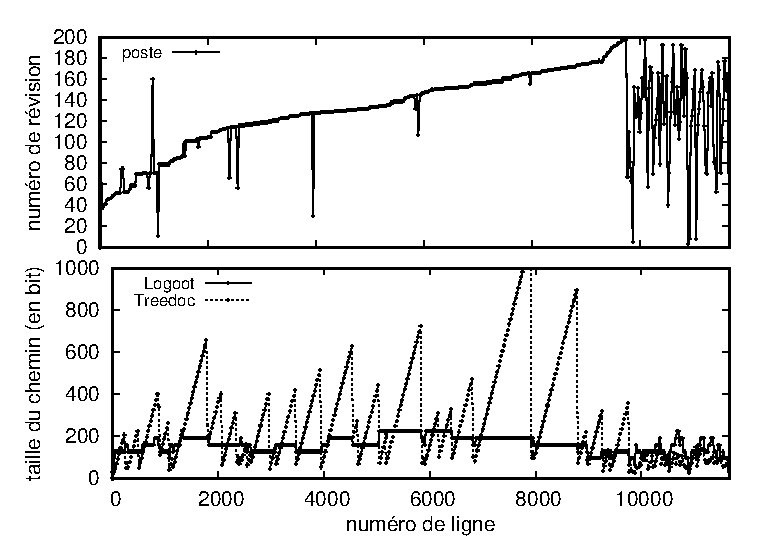
\includegraphics[width=0.8\textwidth]{img/lseq/motivationposte.eps}}
%   \hspace{10pt}
%   \subfloat[Document Wikipédia principalement édité au début]
%   [\label{repl:img:motivationsB}Document Wikipédia de petite taille
%   principalement édité au début.]
%   {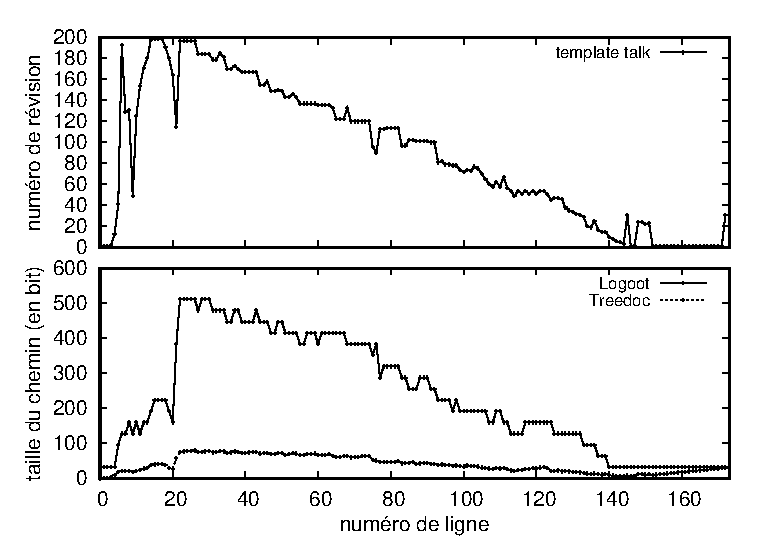
\includegraphics[width=0.8\textwidth]{img/lseq/motivationtemplatetalk.eps}}
%   \caption[Taille du chemin alloué pour chaque ligne dans Wikipédia]
%   {\label{repl:img:motivations} Taille du chemin alloué pour chaque ligne du
%     document. L'axe des abscisses montre le numéro de la ligne concernée. L'axe
%     des ordonnées de la partie haute de la figure montre l'âge de la
%     ligne. L'axe des ordonnées de la partie basse de la figure montre la taille
%     binaire du chemin alloué.}
% \end{figure*}

% L'encyclopédie Wikipédia~\cite{wikipedia} répertorie des millions d'articles
% écrits collaborativement par sa communauté. Un utilisateur, enregistré ou non,
% peut lire un article, et s'il le souhaite, en modifier le contenu. Lorsque ses
% modifications sont achevées, il les soumet à Wikipédia. Deux issues possibles :
% \begin{inparaenum}[(i)]
% \item La contribution est acceptée et sera visible de tous ou
% \item la contribution est rejetée car un autre utilisateur a effectué une
%   modification en concurrence et l'a soumise en premier. Il faut alors réviser
%   la version rejetée afin de l'adapter à la version la plus à jour avant de la
%   soumettre à nouveau, si nécessaire.
% \end{inparaenum}
% Wikipédia garde l'historique des modifications apportées à tous les articles
% depuis leur création. Nous sommes alors à même de rejouer les éditions --
% nommées révision -- dans l'ordre où elles ont été effectuées. Toutefois, la
% concurrence qui pourrait exister dans une édition en temps réelle est effacée
% par le processus d'édition même. D'autre part, la granularité est fixée à la
% ligne. En cela, les simulations sur corpus Wikipédia diffèrent légèrement de la
% réalité.

% \paragraph{Objectif :} Montrer que ni Logoot ni Treedoc ne parviennent pas à
% fournir des identifiants dont la taille soit satisfaisante quel que soit le
% document créé grâce à des traces réelles.

% \paragraph{Description :} Logoot est configuré avec une base $2^{32}$. Treedoc
% est configuré pour utiliser sa méthode originelle -- son autre heuristique
% revenant plus ou moins à la stratégie de Logoot. Les documents considérés sont
% des articles extraits de Wikipédia et rejoués sur 200 révisions. L'un des
% articles atteint jusqu'à 10k lignes principalement ajoutées en fin
% d'article\footnote{\scriptsize\url{https://fr.wikipedia.org/wiki/Liste_des_bureaux_de_poste_français_classés_par_oblitération_Petits_Chiffres}}. L'autre
% article atteint seulement 200 lignes mais est principalement édité en
% tête\footnote{\scriptsize\url{https://en.wikipedia.org/wiki/Template_talk:Did_you_know}}.

% \paragraph{Résultat :} Les figures~\ref{repl:img:motivationsA}
% et~\ref{repl:img:motivationsB} montrent la taille de l'identifiant associé à
% chaque ligne. Nous observons que Treedoc possède des chemins qui augmentent très
% vite quel que soit le type d'édition. Lorsque le nombre d'insertions successives
% est très grand (cf. figure~\ref{repl:img:motivationsA}) les chemins atteignent
% des tailles très élevée dépassant les 1k bits par chemin. Dans ce cas, Logoot se
% comporte mieux. En revanche, dans le cadre de l'édition en tête, Logoot alloue
% des chemins dont la taille augmente extrêmement rapidement. Pour recouvrer de
% bonnes performances, l'exécution d'un protocole de relocalisation des chemins
% devient nécessaire.

% \paragraph{Explication :} Dans les deux types d'édition, Treedoc et Logoot
% allouent des identifiants dont la complexité est linéaire. Ainsi, plus les
% insertions se succèdent, plus l'arbre est déséquilibré, plus la taille du chemin
% augmente. Cependant, comme l'arité des chemins Treedoc est binaire
% ($\mathcal{P}\in \mathbb{N}_{<2}.\mathbb{N}_{<2}\ldots\mathbb{N}_{<2}$), cela
% lui permet de conserver des chemins plus petits que ceux de Logoot dans le cadre
% du document édité en tête. D'un autre coté, Logoot a conçu sa stratégie pour
% l'édition en fin. Dès lors, si le comportement suit cette hypothèse, les
% identifiants grossissent par paliers. Linéairement certes, mais lentement. Dans
% le cas contraire, les identifiants grimpent très rapidement (cela serait le cas
% avec la seconde heuristique de Treedoc).

% \subsubsection{Documents artificiels}


% \begin{figure}
%   \begin{center}
%     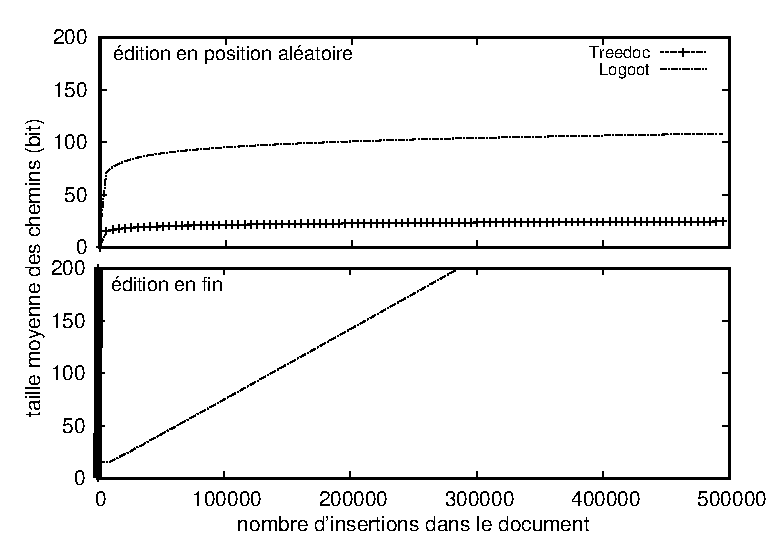
\includegraphics[width=0.8\textwidth]{img/lseq/motivationartificial.eps}
%     \caption[Taille moyenne des chemins sur des documents artificiels]
%     {\label{repl:img:motivationartificial}Taille moyenne des chemins
%       allouées en fonction du nombre d'insertions successives dans le
%       document. L'axe des abscisses montre le nombre d'insertions dans le
%       documents. L'axe des ordonnées montre la taille moyenne de la
%       représentation binaire des chemins alloués.}
%   \end{center}
% \end{figure}

% \paragraph{Objectif :} Montrer la progression de la taille des identifiants
% allouées par les fonctions d'allocation Logoot et Treedoc sur des documents
% artificiels.

% \paragraph{Description :} Deux types de documents artificiels sont créés. Tout
% d'abord, un premier document est créé grâce à des insertions à des positions
% aléatoires dans la séquence. Le second document est créé grâce à des insertions
% successives en fin de document. La fonction d'allocation des chemins de Logoot
% est spécifiquement conçue pour gérer ce dernier type d'édition. La taille
% moyenne des chemins composant les identifiants est mesurée à chaque nouvelle
% insertion. Le document atteint 500k caractères.

% \paragraph{Résultat :} La figure~\ref{repl:img:motivationartificial} montre les
% résultats de cette simulation. La partie du haut montre les résultats du
% document édité à des positions aléatoires. La partie du bas montre les résultats
% du document édité à la fin. Nous observons que l'édition à des positions
% aléatoires entraîne une génération de chemins dont la taille est logarithmique,
% que ce soit pour Logoot ou pour Treedoc. Treedoc est meilleur que Logoot dans ce
% cas. Nous observons aussi que l'édition en fin est catastrophique pour Treedoc
% (la courbe est superposée à l'axe des ordonnées). De son coté, Logoot alloue des
% chemins dont la taille augmente moins rapidement. Malgré cela, la croissance
% reste linéaire. À terme, l'exécution d'un protocole de relocalisation des
% chemins devient nécessaire pour recouvrir de bonnes performances.

% \paragraph{Explication :} Les fonctions d'allocations Logoot et Treedoc
% utilisent une structure d'arbres pour allouer le chemin associé à chaque
% caractère. Dans le cadre de l'édition aléatoire, l'arbre reste équilibré au
% cours des insertions. Les branches les plus basses se remplissent au maximum de
% leur capacité. Par conséquent, les identifiants alloués par Treedoc et Logoot
% croissent logarithmiquement par rapport au nombre d'insertion. L'arité de
% l'arbre de Treedoc étant inférieure à l'arité de l'arbre de Logoot, Treedoc
% propose de meilleures performances. Dans le cadre de l'édition en fin, chaque
% nouvelle insertion dans Treedoc ajoute un bit au chemin généré. La croissance
% est linéaire comparée au nombre d'insertions dans la séquence et extrêmement
% rapide. La fonction d'allocation de Logoot est conçue pour gérer ce type
% d'édition. Une branche par niveau de l'arbre se trouve bien remplie
% d'éléments. Toutefois, le nombre d'éléments accueillis par chaque branche reste
% constant, d'où la croissance linéaire de la taille des chemins générés.


%%% Local Variables:
%%% mode: latex
%%% TeX-master: "../../paper"
%%% End:
